\documentclass[10pt, aspectratio=169]{beamer}
\usetheme{Thesis}

\usepackage[latin1]{inputenc}
\usepackage{amsmath,amsfonts,amssymb}
\usepackage{graphics}
\usepackage{graphicx}
\usepackage{xcolor}
\usepackage{setspace}

\usepackage{multimedia}
\usepackage{media9}
\usepackage{hyperref}
\usepackage{tikz}
\usetikzlibrary{arrows,shapes,shadows,calc}

\setbeamertemplate{itemize/enumerate body begin}{\small}
\setbeamertemplate{itemize/enumerate subbody begin}{\footnotesize}
%\setbeamercovered{transparent}

\setlength{\itemsep}{1ex}




%%%%%%%%%%%%%%%%%%%%%%%%%%%%%%%%%%%%%%%%%%%%%%%
% COLOR Command
\newcommand{\myemph}[1]{\emph{\color{emph@Thesis}#1}}
\newcommand{\mytitle}[1]{\textbf{\color{emph@Thesis}#1}}
\newcommand{\myblue}[1]{{\color{blue@Thesis}#1}}
\newcommand{\myred}[1]{{\color{red@Thesis}#1}}
%%%%%%%%%%%%%%%%%%%%%%%%%%%%%%%%%%%%%%%%%%%%%%%

\title[Control of an autonomous aerodynamic airshield]
  {\Large Control of an autonomous aerodynamic airshield \\
for training Olympics 100m sprint athletes}
\author[Giulia Cutini]{Giulia Cutini}
\institute[University of Bologna]{}
\date{\today}



\graphicspath{{figs/}}


\begin{document}
\footnotesize

%%%%%%%%%%%%%%%%%%%%%%%%%%%%%%%%%%%%%%%%%%%%%%%%%%%%%%%%%%%%%%%%%%%%%%%%%%%%%%%%
%%%%%%%%%%%%%%%%%%%%%%%%%%%%%%%%%%%%%%%%%%%%%%%%%%%%%%%%%%%%%%%%%%%%%%%%%%%%%%%%

\begin{frame}[plain,noframenumbering,t]
\centering

\vspace{0.8cm}
\begin{columns}
\begin{column}{1.1\textwidth}
\centering \footnotesize
\textsc{Alma Mater Studiorum Universit\`{a} di Bologna}\\
\textsc{Department of Electrical, Electronic and Information Engineering}
\\
\vspace{0.2cm}
\textsc{Master's Degree in Automation Engineering}
\end{column}
\end{columns}

\vspace{0.5cm}

\textcolor{blue@Thesis}{\Large \bf \inserttitle}

\vspace{1cm}

\begin{columns}[t]
\begin{column}{0.5\textwidth}
	\myemph{Candidate:}
	
	\hspace{0.5cm} Giulia Cutini
\end{column}

\begin{column}{0.4\textwidth}
	\myemph{Advisor:}
	
		\hspace{0.5cm} Prof.~Giuseppe Notarstefano
		
		\vspace{.4cm}
		\myemph{Co-Advisors:}
	
		\hspace{0.5cm} Prof.~Melanie Zeilinger \\
		\hspace{0.5cm} Dr.~Andrea Carron \\
		\hspace{0.5cm} Ing.~Lorenzo Sforni
\end{column}
	
\end{columns}

\begin{tikzpicture}[remember picture,overlay]
\node[anchor=south west,inner sep=0pt] at (current page.south west) {
	\hspace{1cm} 
\includegraphics[height=1.5cm]{Logo_unibo}
};
\node[anchor=south east,inner sep=0pt] at (current page.south east) {
	
\includegraphics[height=0.8cm]{Logo_ETH}  \hspace{1cm} 
};
\end{tikzpicture}

\vspace{0.5cm}
\begin{center}
\scriptsize
  \textcolor{emph@Thesis}{Bologna, 18 March 2024}
\end{center}
\end{frame}


\begin{frame}
\frametitle{Table of Contents}
\begin{itemize}
	\footnotesize
	\item[$\blacktriangleright$]<1-> Introduction
		\begin{itemize}
			\footnotesize
			\setstretch{1.2}
			\item[$\triangleright$]<1-> Motivations
			\item[$\triangleright$]<1-> Contributions
		\end{itemize}
	\item[$\blacktriangleright$]<2-> Modeling of the go-kart with the airshield attached
	\item[$\blacktriangleright$]<3-> Control design
		\begin{itemize}
			\footnotesize
			\setstretch{1.2}
			\item[$\triangleright$]<3-> Gain Scheduling Linear Quadratic Regulator
			\item[$\triangleright$]<3-> Model Predictive Control
			\item[$\triangleright$]<3-> Offset-free Model Predictive Control
		\end{itemize}
	\item[$\blacktriangleright$]<4-> Simulation test and numerical controllers comparison
	\item[$\blacktriangleright$]<5-> Hardware-in-the-loop tests
\end{itemize}
\end{frame}

%%% First frame
\begin{frame}[t]
\frametitle{Introduction}
\vspace{0.1cm}
\textcolor{emph@Thesis}{\textbf{\small{Motivations}}} \\
\vspace{0.3cm}
\onslide<1,2,3>In athletics, the \textbf{overspeed training} makes possible to enhance the competition performances.

\setstretch{1.3}
\onslide <1,2,3>It can be achieved by isolating the runner from the air resistance using an \textbf{airshield}.

\begin{columns}
\hspace{0.2cm}
\begin{column}{0.48\textwidth}
\footnotesize
\setstretch{0.4}
\onslide <2,3>The usage of an \textbf{autonomous go-kart} improves:
	\begin{itemize}
		\footnotesize
		\item[$\blacktriangleright$] <2->the safety of the maneuver
		\item[$\blacktriangleright$] <2->the reliability and the reusability 
	\end{itemize}
\end{column}
\begin{column}{0.52\textwidth}
	\begin{center}
  		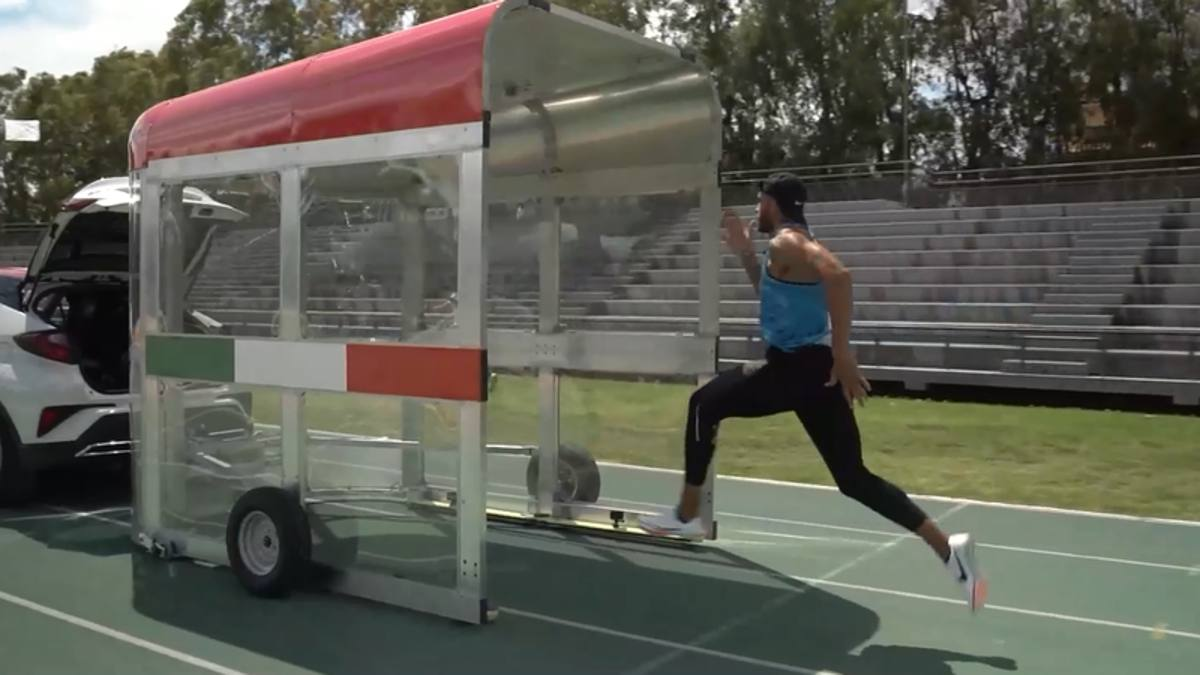
\includegraphics[width=0.48\textwidth]{Jacobs} 
		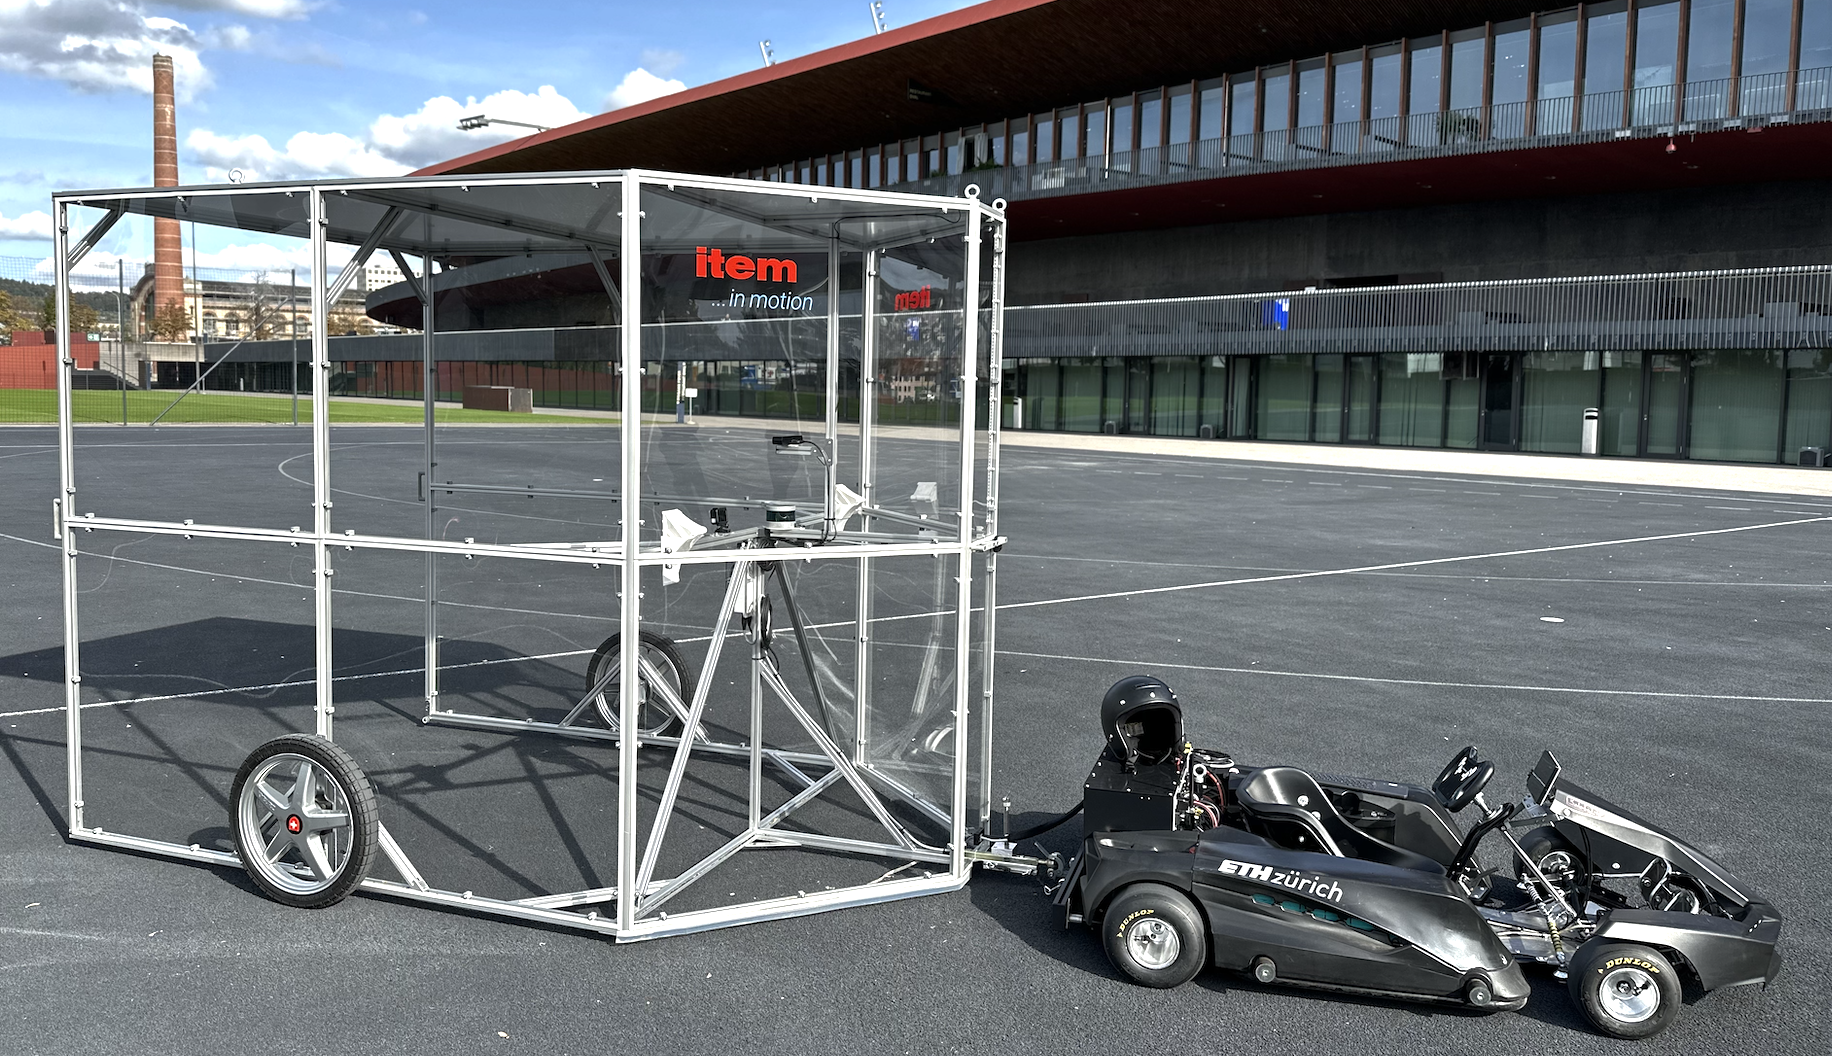
\includegraphics[width=0.47\textwidth]{Windshield} 
	\end{center}
\end{column}
\end{columns}
\vspace{0.3cm}

\onslide <3> \textcolor{emph@Thesis}{\textbf{\small{Contributions}}} \\
\vspace{0.1cm}
\footnotesize
\begin{itemize}
	\setstretch{1.0}
	\footnotesize
	\item[$\blacktriangleright$] <3->Model of the system: the autonomous go-kart with the airshield attached
	\item[$\blacktriangleright$] <3->Design a controller for the system to regulate it with respect to the runner
	\item[$\blacktriangleright$] <3->Test the controller
\end{itemize}
\end{frame}


%%% Second frame
\begin{frame}[t]
\frametitle{Modeling of the go-kart with the aishield attached}
%\vspace{0.2cm}
\begin{columns}
\begin{column}{0.4\textwidth}
	\begin{center}
  		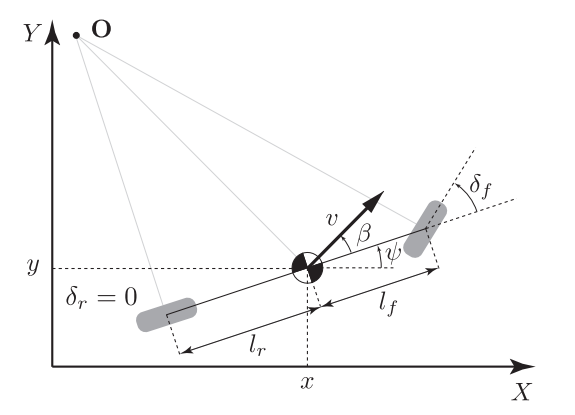
\includegraphics[width=0.75\textwidth]{Bycicle_scheme} 
	\end{center}
\end{column}
%\vspace{0.1cm}
\begin{column}{0.6\textwidth}
\onslide <1,2,3,4,5,6,7> \textbf{Non linear kinematic byclicle model}
	\begin{equation*}
	\begin{cases}
 		\begin{aligned}
			\dot{x}(t) &= v(t) \cos(\psi(t) + \beta(t)) \\
			\dot{y}(t) &= v(t) \sin(\psi(t) + \beta(t)) \\
			\dot{\psi}(t) &= \frac{v(t)}{l_r} \sin(\beta(t)) \\
			\dot{v}(t) &= \frac{F_x(t)}{m} = \frac{1}{m} (C_{m1}a(t) - C_f v(t) - \alert<5,6>{C_d v^2(t) - C_{roll}}) \\
		\end{aligned}
	\end{cases}
	\end{equation*}
\end{column}
\end{columns}

\vspace{0.4cm}

\begin{columns}
\begin{column}{0.5\textwidth}
\hspace{0.8cm} 
\onslide <2,3,4,5,6,7> The runners are interested in executing \\
\hspace{0.9cm} only 50-80 meters overspeed training 
\end{column}
\begin{column}{0.1\textwidth}
\onslide <3,4,5,6,7> $\Rightarrow$
\end{column}
\begin{column}{0.4\textwidth}
\hspace{-0.5cm}
\onslide <4,5,6,7> The model can be simplified \\
\hspace{-0.6cm} by not considering the steering
\end{column}
\end{columns}

\vspace{0.6cm}

\begin{columns}
\hspace{0.8cm}
\begin{column}{0.4\textwidth}
\vspace{-0.5cm}
\onslide <5,6,7>\begin{equation*}
	\begin{cases}
 	\begin{aligned}
		\dot{p}(t) &= v(t) \\
		\dot{v}(t) &= \frac{F(t)}{m} = \frac{1}{m} (C_{m1} a(t) - C_f v(t) \onslide<5,6>{- \alert<6>{C_d v^2(t) - C_{roll}})}
	\end{aligned}
	\end{cases}
\end{equation*}
\end{column}

\begin{column}{0.6\textwidth}
\onslide<7>\begin{equation*}
    \begin{aligned}
    	x_{k,t+1} = 
    		\begin{bmatrix}
    			p_{k,t+1} \\
    			v_{k,t+1}
    		\end{bmatrix}
    		& =
    		\begin{bmatrix}
    			1 & dt \\
    			0 & 1-dt\frac{C_f}{m}
    		\end{bmatrix}
    		x_{k,t}
    		+
    		\begin{bmatrix}
    			0 \\
    			dt \frac{C_{m1}}{m}
    		\end{bmatrix}
    		u_t \\
    		& = A \, x_{k,t} + B \, u_t
    \end{aligned}
\end{equation*}
\onslide<7> \hspace{2.5cm}\textbf{Linear time-invariant system}
\end{column}
\end{columns}
\hspace{0.4cm}
\vspace{0.4cm}
\onslide<6>The non linear term can be removed

\end{frame}

\section{Control design}
\subsection{Linear Quadratic Regulator}
\begin{frame}[t]
\frametitle{Gain Scheduling Linear Quadratic Regulator}
\end{frame}


\subsection{Model Predictive Control}
\begin{frame}
\frametitle{Model Predictive Control}
\end{frame}


\subsection{Offset-free Model Predictive Control}
\begin{frame}
\frametitle{Offset-free Model Predictive Control}
Cio
\end{frame}

\section{Simulation tests and Controllers comparison}
\begin{frame}
\frametitle{Simulation tests and Controllers comparison}
\end{frame}


\begin{frame}
\frametitle{Hardware-in-the-loop tests}
%\begin{centering}
%	\movie[externalviewer,loop,poster]{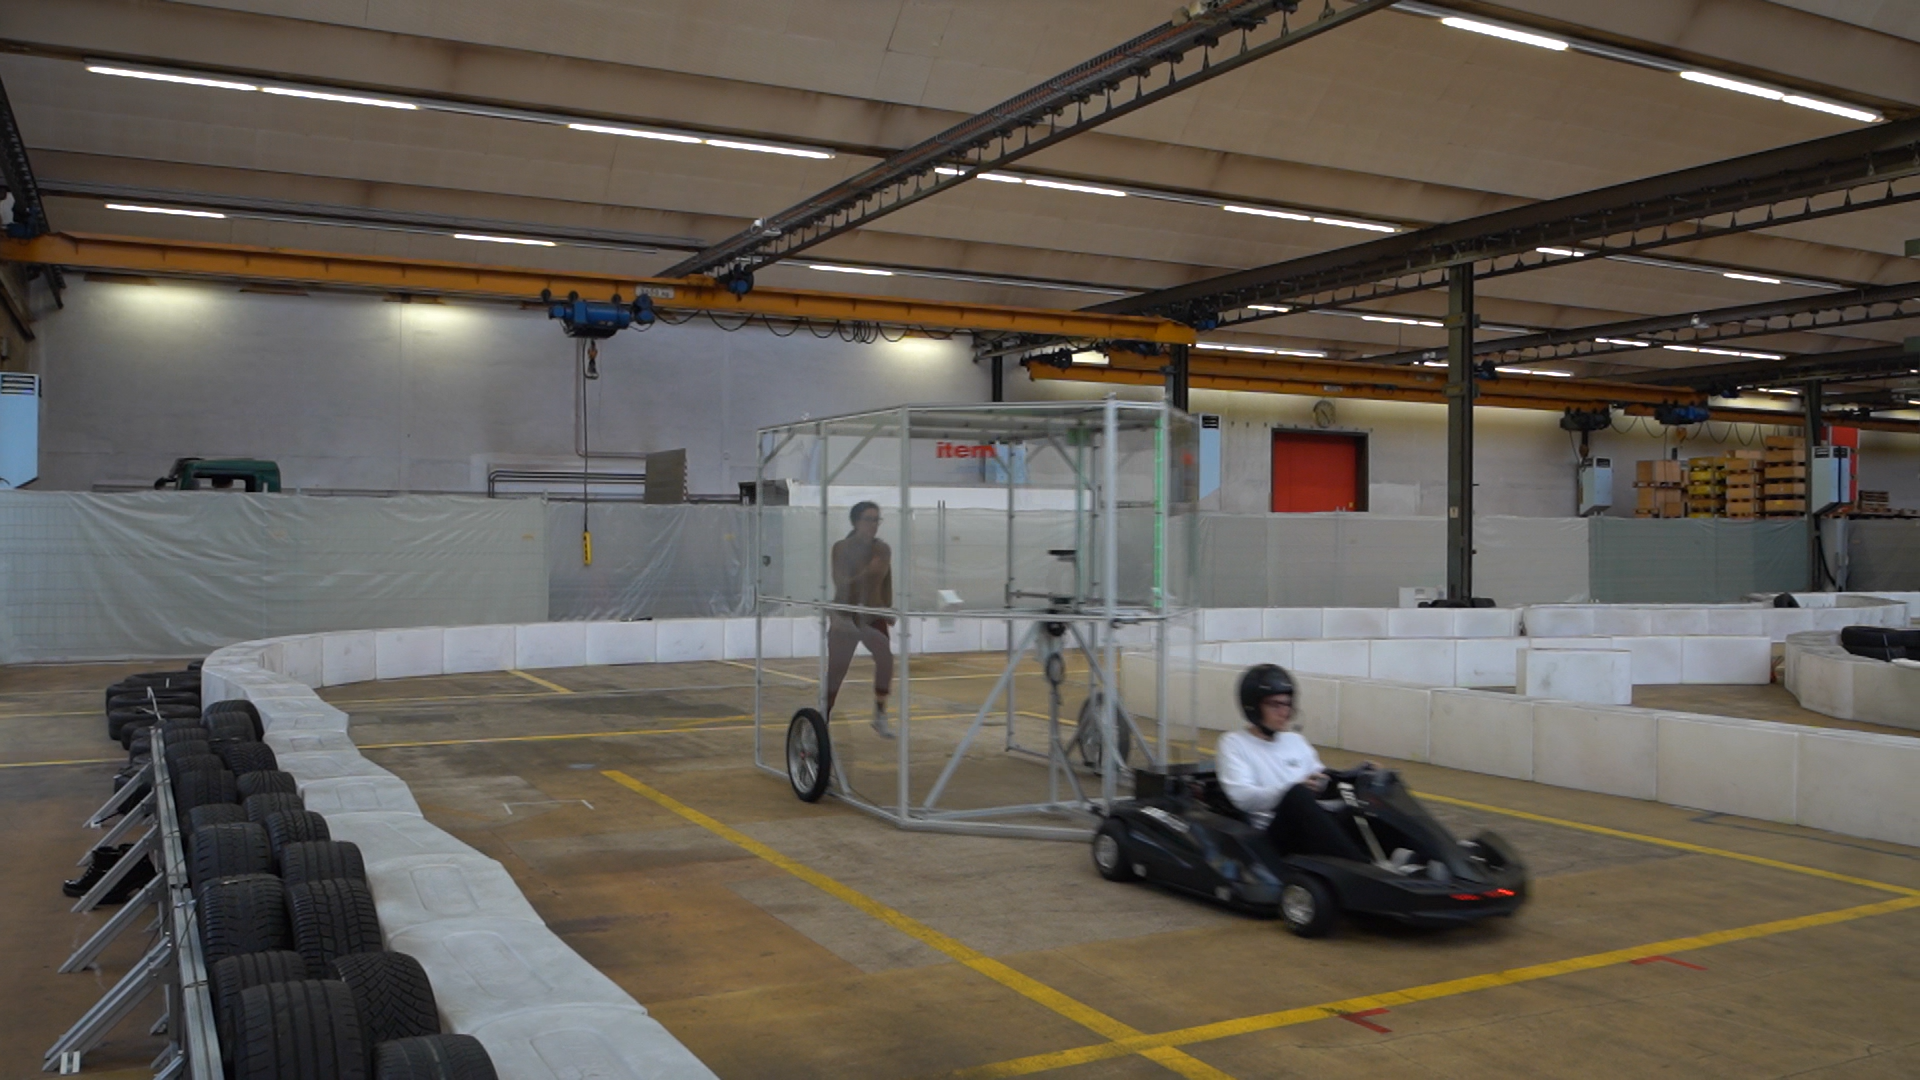
\includegraphics[width=0.8\textwidth, keepaspectratio]{Poster}}{video.mp4}
%\end{centering}

\begin{center}
\href{video.mp4}{
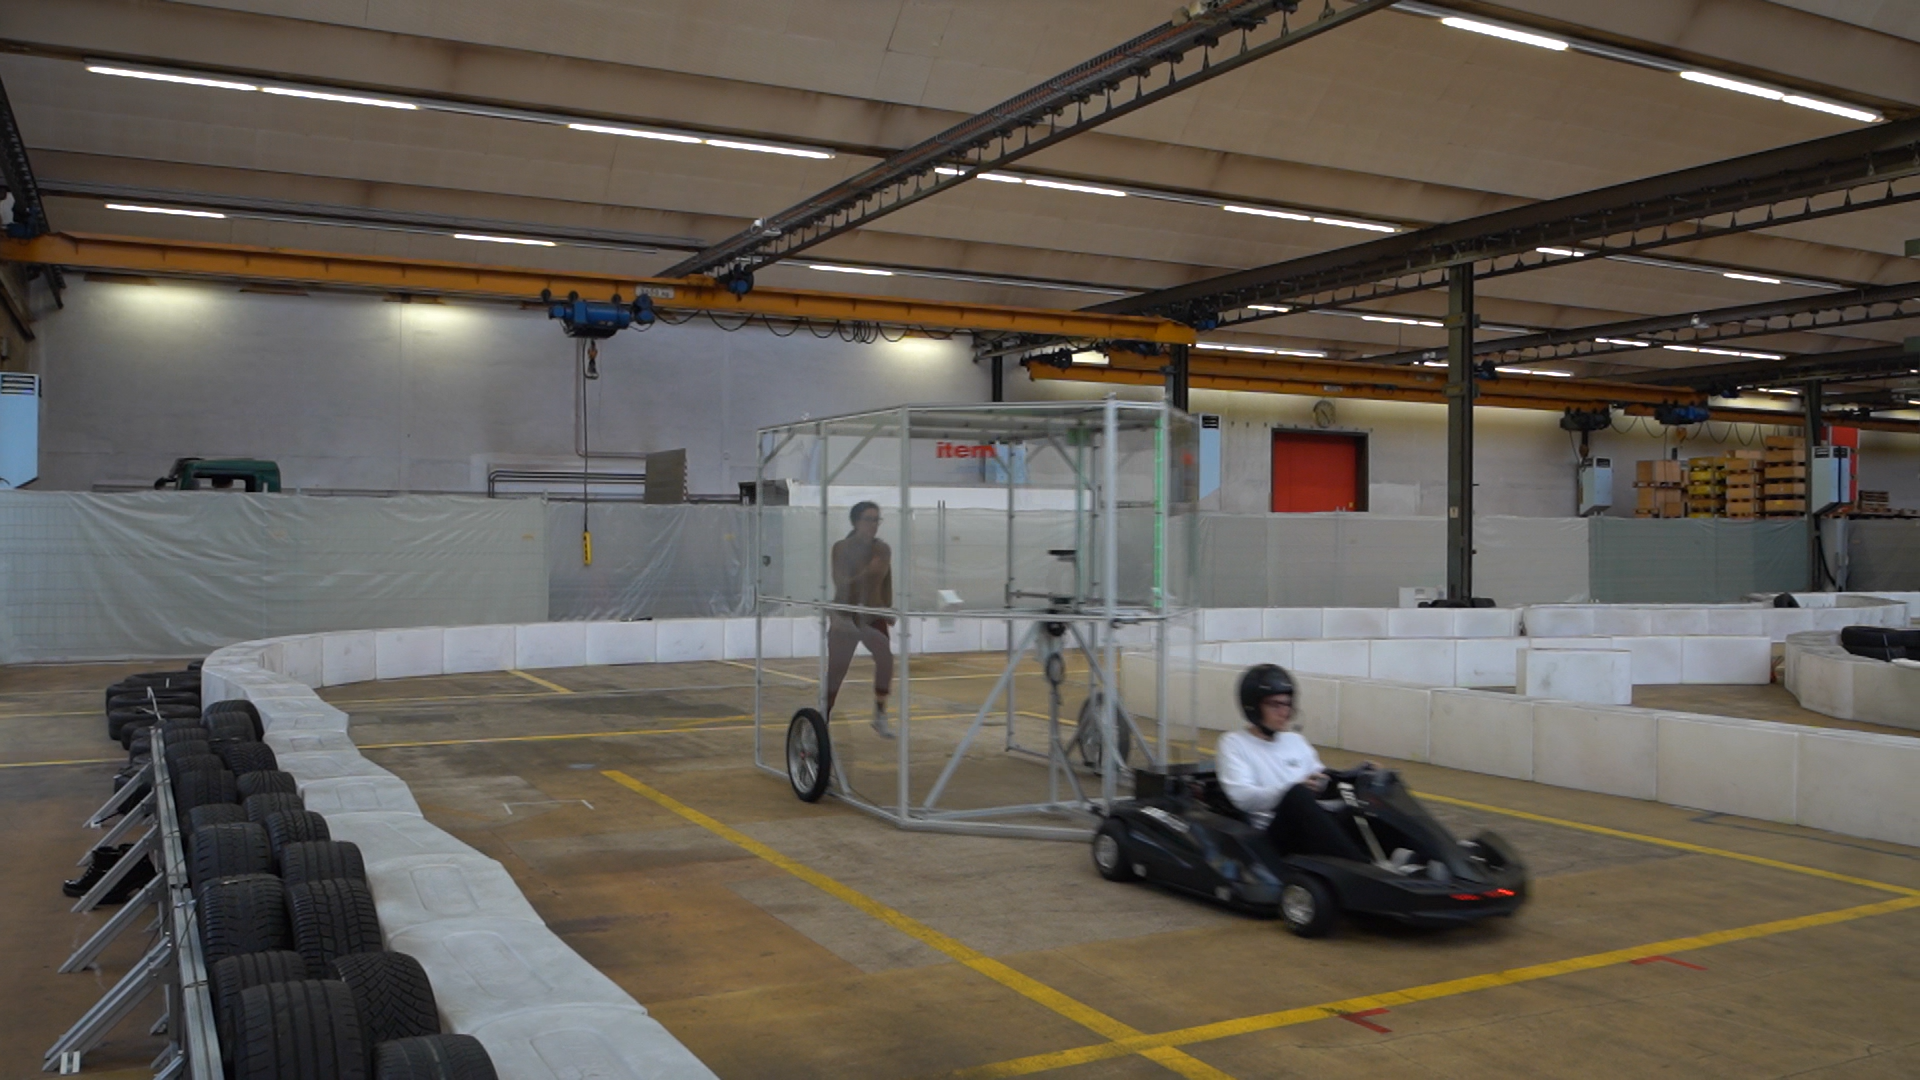
\includegraphics[scale=0.25]
{Poster}}
\end{center}
\end{frame}
\end{document}

\begin{columns}
\begin{column}{0.5\linewidth}


Some text
%
\begin{itemize}
\item Bullet 1
\item Bullet 2
\item Bullet 3
\end{itemize}

\end{column}
%
\begin{column}{0.5\textwidth}

\begin{center}
  \includegraphics[scale=1]{example_figure.pdf}
\end{center}

\end{column} 
\end{columns}

\vspace{1cm}
An equation
\begin{align*}
\dot{x} = f(x,u)
\end{align*}


